\section{Background}
\subsection{A Closer Look At The Problem}
To get a better understanding of the problem Optika is trying to solve, it is
best to look at an example of said problem. Currently, the program Tramonto has
a massive input file filled with complex, non-intuitive inputs. Below
\ref{tramontoInputFigure} is just small section of this input file.
\begin{figure}
  \centering
  {\footnotesize
  \begin{verbatim}
************* DIMENSION PARAMETERS ********************************************
@ -1. -1. -1. -1. 10. 	Length_ref Density_ref Temp Dielec_ref VEXT_MAX 
************* MESH PARAMETERS *************************************************
@ 3 	Ndim 
@ 3. 2. 2. 	Size_x(idim): idim=0,Ndim-1 
@ 0.25 0.25 0.25 	Esize_x(idim): idim=0,Ndim-1 
@ -1 2 	Type_bc(x0,: left, right) (-1=IN_WALL, 0=IN_BULK, 1=PERIODIC, 2=REFLECT, 3=LAST_NODE) 
@ 1 1 	Type_bc(x1,: down, up) 
@ 1 1 	Type_bc(x2,: back, front) 
  \end{verbatim}
  }
  \caption[Tramonto Input]{An example of the complex input file used by Tramonto}
  \label{tramontoInputFigure}
\end{figure}
This input file is hard to read and non-intutive, not to mention it could 
easily intimidate
a new user. In fact, Tramonto's current input system is so complicated, 
that it is recommended most users simply take sample input files and just 
modify them for their needs.

\subsection{Why Not Something Else?}
Instead of relying on current solutions GUI solutions to solve the above problem, Optika was created in order to address
a number of constraints.
\subsubsection{Something Simple}
Current GUI frameworks like Qt (on which Optika is based), GTK+, and Cocao are incredibly roboust. But
because of this they are also large and complicated. When looking for a solution to the 
scientific application interface problem, we need something that is simple. Otherwise, as mentioned
above, developers will be hesistent to use it.

\subsubsection{Cross-Platform}
Having a better user interface can lead to having a wider user base. When adding the functionality
of a GUI to your application, you don't want to accidentally exclude some of your users by
using a technology that won't work on their platform of choice. Cocao for example only works on
Mac OSX systems. By using Qt as it's underpinnings, Optika is able to work on a wide variety of
platforms.

\subsubsection{Trilinos Integration}
Optika was developed as part of the Trilinos project. Trilinos is a set of C++ libraries
used extensively throughout the scientific community. Since Optika is part of Trilinos,
we wanted it to have tight integration with constucts that were already in place inside
of Trilinos. By creating our own GUI solution, Optika allows users already familiar
with the Trilinos framework to take advantage of the capabilities Optika has to offer.

\section{Optika Overview}
\subsection{GUI Fundamentals}
An Optika based GUI is laid out in a hirerachical fashinon as shown in Figure \ref{paramlistFigure}.
This hierachy is made up of Parameters and ParameterLists. Parameters can simply be thought of as single input for
a program. A ParameterList is simply a collection of Parametes and other ParameterLists. When a ParameterList
is part of another ParameterList we call it a sublist.
		\begin{figure}
			\centering
			\begin{picture}(50,150)(0,0)
				\put(10,0){\line(0,1){145}}
				\put(0,150){${Parameter List}$}
				\put(10,130){\line(1,0){15}}
				\put(28,127){$Parameter$}
				\put(10,110){\line(1,0){15}}
				\put(28,107){$Parameter$}
				\put(10,90){\line(1,0){15}}
				\put(28,87){$Parameter$}
				\put(10,70){\line(1,0){15}}
				\put(28,67){$Parameter List$}
				\put(38,0){\line(0,1){62}}
				\put(38,47){\line(1,0){15}}
				\put(56,44){$Parameter$}
				\put(38,22){\line(1,0){15}}
				\put(56,24){$Parameter$}
			\end{picture}
			\caption[GUI Layout]{The hierarchical layout of the GUI}
			\label{paramlistFigure}
		\end{figure}

Parameters in Optika are typed. Parameters can be any one of the following types:
  \begin{multicols}{2}
		\begin{itemize}
			\item int
			\item short
			\item float
			\item double
			\item string
			\item boolean
			\item arrays of int, short, double, and string
		\end{itemize}
	\end{multicols}
When editing a parameter in Optika different ``widgets'' are used to change the parameters value. A widget is simply
a graphical construct used for obtaining input from the user. For number types, a spin box (Figure~\ref{spinboxfig}) is used to obtain input. 
If the valid values for a string type were specified (something that will be discussed later), a combo box (Figure~\ref{comboboxfig}) is used.
Otherwise a line edit (Figure~\ref{lineeditfig}) is used to edit a string parameters. For booleans, a combo box (Figure~\ref{comboboxfig}) 
is also be used. For arrays, a pop-up box containing numerous input widgets is used. The widget type is determined by the
array type (e.g. for numerical types a series of spinboxes would be used, for string types comboxes or lineedits are used, etc.). 
	\begin{figure}
		\centering
		\subfigure[A Spin Box]{
			\label{spinboxfig}
			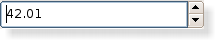
\includegraphics[scale=0.5]{graphics/spinbox}
		}
		\subfigure[A Combo Box]{
			\label{comboboxfig}
			
\includegraphics[scale=0.5]{graphics/combobox}
		}
		\subfigure[A Line Edit]{
			\label{lineeditfig}
			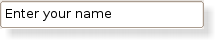
\includegraphics[scale=0.5]{graphics/lineedit}
		}
		\caption{Some of the various widgets used for editing data~\cite{QtGallery}}
		\label{editingWidgets}
	\end{figure}
When you put it all together a basic Optika GUI looks something like Figure~\ref{basicexample}.
When the user clicks on a particular value, one of the above widgets pops up allowing them to edit the value.
  \begin{figure}
  \centering
  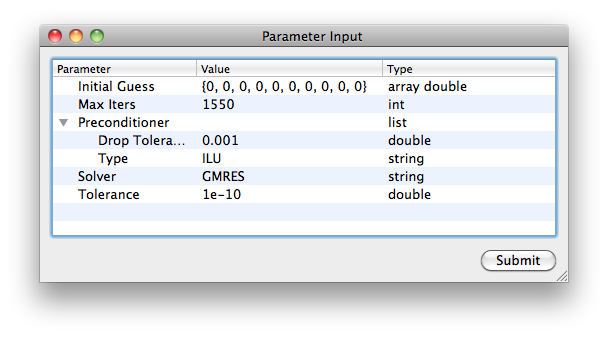
\includegraphics[scale=0.5]{graphics/basic_example}
  \label{basicexample}
  \caption[Basic GUI]{A basic Optika GUI}
  \end{figure} 
\subsection{Underlying Technologies}
Optika is one of many packages in the Trilinos project~\cite{trilinos}, which is developed by Sandia National Labs. At it's core, 
the Trilinos project is a collection of various
libraries for aiding developers of scientific applications. Trilinos is best known for it's extensive colleciton of equation solvers,
but also provides a wealth of other tools that support general high performance computing. Each package in the Trilinos project provides
it's own set of unique capabilities. Optika is Trilnos's GUI package.

In order to provide GUI funcitonality, Optika relies on the Qt Framework~\cite{Qt}. 
Qt was choosen as Optika's backing GUI framework for several
reasons:
	\begin{itemize}
		\item It is cross-platform, allowing Optika to be used in many different computing environments.
		\item It is mature and has a comprehensive set of development tools. So we don't have to worry about major bugs.
		\item It has a rich feature-set, permiting Optika to grow in it's capbilities if necessary.
    \item It has a large user base.
		\item It has been used by Sandia in the past.
		\item The Optika lead developer was familiar with it.
	\end{itemize}
Because Trilinos is itself a library, relying on an additional third-party library can be a risky endevour. But
the qualities outlined above made using Qt a very easy choice. When choosing to use Qt we felt very confident that we 
would be able to rely on it to be stable, and to provide us with the tools we needed.

In order to configure and build Optika, the CMake~\cite{cmake} build system is used. This is actually the build system
used by Trilinos as a whole, so it makes perfect sense for Optika to use it as well. In addition, CMake
has support for the necessary special building tools required by Qt.

\section{Using Optika}
At the core of Optika is the ParameterList class from the Teuchos package~\cite{TeuchosPackage}, another part
of the Trilinos project. ParameterLists can be constructed either from within C++ source code or using XML.
In this paper, we will first start off with basic examples using C++ source code. However, once we start
talking about the more complex features we'll switch over to XML.
\subsection{Basic Usage}
Since Tramonto is so sorely lacking in a quality user interface, we'll use it as an example of how to use Optika.
Let's look at the Dimenstion Control Parameters. These are just a few parameters used to define what kind of
dimensions are going to be used in the rest of the input file. Figure~\ref{basicTramonto} shows how we would create
such a GUI.

\begin{figure}
\centering
\lstinputlisting[language=C++, basicstyle=\scriptsize]{basicTramonto/main.cpp}
\label{basicTramonto}
\caption{Basic Tramonto Example}
\end{figure}

We start by including the Optika\_GUI.hpp file. This include file allows us to use most of Optika's basic functionality.
Once in the main function we import several classes and functions into the namespace. We then create two
ParameterList RCPs\footnote{For more information on RCPs see~\cite{RCP}}. Using the sublist function, the second 
ParameterList is defined as a sublist of the first. The next several lines are calls to the set function. Each call
adds a Parameter to the ParameterList along with assigning it a default value and a documentation string. The end result
is Figure~\ref{BasicTramontoScreenShot}.

\begin{figure}
\centering
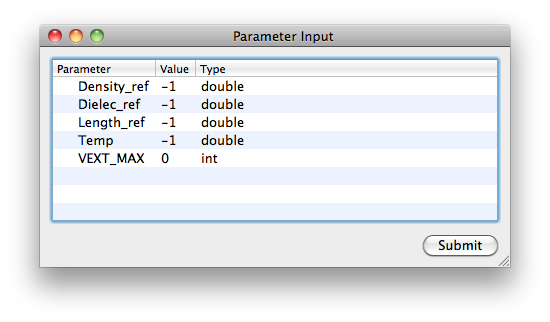
\includegraphics[scale=0.5]{graphics/BasicTramontoScreenshot}
\label{BasicTramontoScreenshot}
\caption{The find product of the code in Figure~\ref{basicTramonto}}
\end{figure}

\subsection{Utilizing XML}
Using XML to declare your input parameters has a number of advantages over declaring you input in C++ source code.
\begin{itemize}
  \item XML is a lot cleaner than the corresponding C++. The source code approach can get pretty unruly, especially
  when some of the more advanced features of Optika are used.
  \item As an extension of being cleaner, using XML makes maintaining a user interface much simpler.
  \item When using XML, there is no need to recompile the entire program everytime a small change is made to the GUI.
\end{itemize}

